\documentclass[twoside]{book}

% Packages required by doxygen
\usepackage{fixltx2e}
\usepackage{calc}
\usepackage{doxygen}
\usepackage{graphicx}
\usepackage[utf8]{inputenc}
\usepackage{makeidx}
\usepackage{multicol}
\usepackage{multirow}
\PassOptionsToPackage{warn}{textcomp}
\usepackage{textcomp}
\usepackage[nointegrals]{wasysym}
\usepackage[table]{xcolor}

% Font selection
\usepackage[T1]{fontenc}
\usepackage{mathptmx}
\usepackage[scaled=.90]{helvet}
\usepackage{courier}
\usepackage{amssymb}
\usepackage{sectsty}
\renewcommand{\familydefault}{\sfdefault}
\allsectionsfont{%
  \fontseries{bc}\selectfont%
  \color{darkgray}%
}
\renewcommand{\DoxyLabelFont}{%
  \fontseries{bc}\selectfont%
  \color{darkgray}%
}
\newcommand{\+}{\discretionary{\mbox{\scriptsize$\hookleftarrow$}}{}{}}

% Page & text layout
\usepackage{geometry}
\geometry{%
  a4paper,%
  top=2.5cm,%
  bottom=2.5cm,%
  left=2.5cm,%
  right=2.5cm%
}
\tolerance=750
\hfuzz=15pt
\hbadness=750
\setlength{\emergencystretch}{15pt}
\setlength{\parindent}{0cm}
\setlength{\parskip}{0.2cm}
\makeatletter
\renewcommand{\paragraph}{%
  \@startsection{paragraph}{4}{0ex}{-1.0ex}{1.0ex}{%
    \normalfont\normalsize\bfseries\SS@parafont%
  }%
}
\renewcommand{\subparagraph}{%
  \@startsection{subparagraph}{5}{0ex}{-1.0ex}{1.0ex}{%
    \normalfont\normalsize\bfseries\SS@subparafont%
  }%
}
\makeatother

% Headers & footers
\usepackage{fancyhdr}
\pagestyle{fancyplain}
\fancyhead[LE]{\fancyplain{}{\bfseries\thepage}}
\fancyhead[CE]{\fancyplain{}{}}
\fancyhead[RE]{\fancyplain{}{\bfseries\leftmark}}
\fancyhead[LO]{\fancyplain{}{\bfseries\rightmark}}
\fancyhead[CO]{\fancyplain{}{}}
\fancyhead[RO]{\fancyplain{}{\bfseries\thepage}}
\fancyfoot[LE]{\fancyplain{}{}}
\fancyfoot[CE]{\fancyplain{}{}}
\fancyfoot[RE]{\fancyplain{}{\bfseries\scriptsize Generated on Sun Dec 7 2014 12\+:20\+:23 for Key\+Player by Doxygen }}
\fancyfoot[LO]{\fancyplain{}{\bfseries\scriptsize Generated on Sun Dec 7 2014 12\+:20\+:23 for Key\+Player by Doxygen }}
\fancyfoot[CO]{\fancyplain{}{}}
\fancyfoot[RO]{\fancyplain{}{}}
\renewcommand{\footrulewidth}{0.4pt}
\renewcommand{\chaptermark}[1]{%
  \markboth{#1}{}%
}
\renewcommand{\sectionmark}[1]{%
  \markright{\thesection\ #1}%
}

% Indices & bibliography
\usepackage{natbib}
\usepackage[titles]{tocloft}
\setcounter{tocdepth}{3}
\setcounter{secnumdepth}{5}
\makeindex

% Hyperlinks (required, but should be loaded last)
\usepackage{ifpdf}
\ifpdf
  \usepackage[pdftex,pagebackref=true]{hyperref}
\else
  \usepackage[ps2pdf,pagebackref=true]{hyperref}
\fi
\hypersetup{%
  colorlinks=true,%
  linkcolor=blue,%
  citecolor=blue,%
  unicode%
}

% Custom commands
\newcommand{\clearemptydoublepage}{%
  \newpage{\pagestyle{empty}\cleardoublepage}%
}


%===== C O N T E N T S =====

\begin{document}

% Titlepage & ToC
\hypersetup{pageanchor=false,
             bookmarks=true,
             bookmarksnumbered=true,
             pdfencoding=unicode
            }
\pagenumbering{roman}
\begin{titlepage}
\vspace*{7cm}
\begin{center}%
{\Large Key\+Player }\\
\vspace*{1cm}
{\large Generated by Doxygen 1.8.8}\\
\vspace*{0.5cm}
{\small Sun Dec 7 2014 12:20:23}\\
\end{center}
\end{titlepage}
\clearemptydoublepage
\tableofcontents
\clearemptydoublepage
\pagenumbering{arabic}
\hypersetup{pageanchor=true}

%--- Begin generated contents ---
\chapter{Hierarchical Index}
\section{Class Hierarchy}
This inheritance list is sorted roughly, but not completely, alphabetically\+:\begin{DoxyCompactList}
\item P\+Applet\begin{DoxyCompactList}
\item \contentsline{section}{keyplayer\+\_\+gui}{\pageref{classkeyplayer__gui}}{}
\end{DoxyCompactList}
\end{DoxyCompactList}

\chapter{Class Index}
\section{Class List}
Here are the classes, structs, unions and interfaces with brief descriptions\+:\begin{DoxyCompactList}
\item\contentsline{section}{\hyperlink{classkeyplayer__gui}{keyplayer\+\_\+gui} }{\pageref{classkeyplayer__gui}}{}
\end{DoxyCompactList}

\chapter{Class Documentation}
\hypertarget{classkeyplayer__gui}{\section{keyplayer\+\_\+gui Class Reference}
\label{classkeyplayer__gui}\index{keyplayer\+\_\+gui@{keyplayer\+\_\+gui}}
}
Inheritance diagram for keyplayer\+\_\+gui\+:\begin{figure}[H]
\begin{center}
\leavevmode
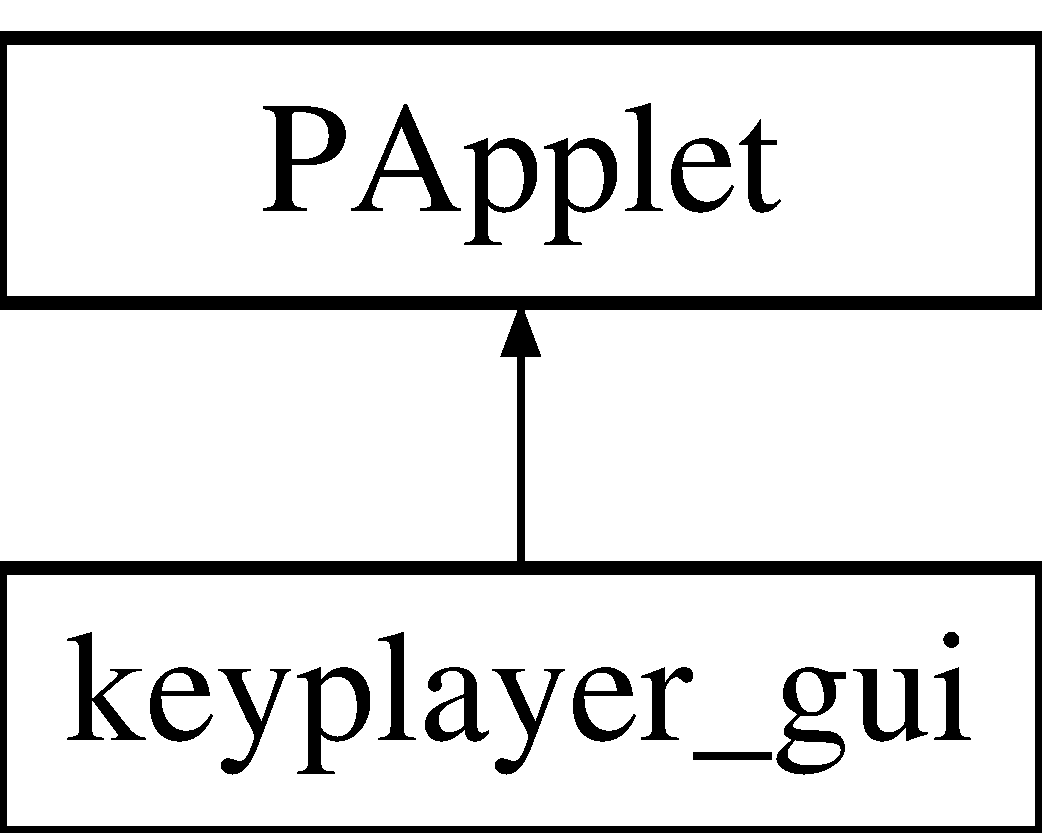
\includegraphics[height=2.000000cm]{classkeyplayer__gui}
\end{center}
\end{figure}
\subsection*{Public Member Functions}
\begin{DoxyCompactItemize}
\item 
void \hyperlink{classkeyplayer__gui_a4f51c3d761204be4bc5ba4f48e806e41}{setup} ()
\item 
void \hyperlink{classkeyplayer__gui_ae66ace1d0588e8896343b325869eb470}{draw} ()
\item 
void \hyperlink{classkeyplayer__gui_a11a22f0316258cecae2fd0cca0ffb066}{key\+Pressed} ()
\item 
void \hyperlink{classkeyplayer__gui_a4c150bd38043603ea0fb728e613f280d}{key\+Released} ()
\item 
void \hyperlink{classkeyplayer__gui_a70e441c8e0a91ac353fc89ef9b3b98bf}{stop} ()
\item 
\hypertarget{classkeyplayer__gui_a2aa16036156f3c1162cbb5ed914b6d0e}{void {\bfseries custom\+G\+U\+I} ()}\label{classkeyplayer__gui_a2aa16036156f3c1162cbb5ed914b6d0e}

\item 
\hypertarget{classkeyplayer__gui_af27ee7b976b3ca3c7904eeaf8997398c}{void {\bfseries q\+\_\+click1} (G\+Button source, G\+Event event)}\label{classkeyplayer__gui_af27ee7b976b3ca3c7904eeaf8997398c}

\item 
\hypertarget{classkeyplayer__gui_a9bd46c0099801f8bf028098851413689}{void {\bfseries w\+\_\+click1} (G\+Button source, G\+Event event)}\label{classkeyplayer__gui_a9bd46c0099801f8bf028098851413689}

\item 
\hypertarget{classkeyplayer__gui_a7841852b38e4abd997b8d3ded6ac20ba}{void {\bfseries e\+\_\+click1} (G\+Button source, G\+Event event)}\label{classkeyplayer__gui_a7841852b38e4abd997b8d3ded6ac20ba}

\item 
\hypertarget{classkeyplayer__gui_af61b8f4a996c76e6cfe90d8a988c0be6}{void {\bfseries r\+\_\+click1} (G\+Button source, G\+Event event)}\label{classkeyplayer__gui_af61b8f4a996c76e6cfe90d8a988c0be6}

\item 
\hypertarget{classkeyplayer__gui_a3455aeebb5d53bcfd236be172961244b}{void {\bfseries slider1\+\_\+change1} (G\+Slider source, G\+Event event)}\label{classkeyplayer__gui_a3455aeebb5d53bcfd236be172961244b}

\item 
\hypertarget{classkeyplayer__gui_aaec3693f64267b2053912dcf4fd32660}{void {\bfseries t\+\_\+click1} (G\+Button source, G\+Event event)}\label{classkeyplayer__gui_aaec3693f64267b2053912dcf4fd32660}

\item 
\hypertarget{classkeyplayer__gui_ae84deb0013362301f9ee8b452b264c48}{void {\bfseries y\+\_\+click1} (G\+Button source, G\+Event event)}\label{classkeyplayer__gui_ae84deb0013362301f9ee8b452b264c48}

\item 
\hypertarget{classkeyplayer__gui_a22be19d2a4aa29c91b1888859856aefc}{void {\bfseries u\+\_\+click1} (G\+Button source, G\+Event event)}\label{classkeyplayer__gui_a22be19d2a4aa29c91b1888859856aefc}

\item 
\hypertarget{classkeyplayer__gui_adbd617bd30824da78b036a048f142592}{void {\bfseries i\+\_\+click1} (G\+Button source, G\+Event event)}\label{classkeyplayer__gui_adbd617bd30824da78b036a048f142592}

\item 
\hypertarget{classkeyplayer__gui_a51ef4d997c462d761de6e64118bd58f9}{void {\bfseries a\+\_\+click1} (G\+Button source, G\+Event event)}\label{classkeyplayer__gui_a51ef4d997c462d761de6e64118bd58f9}

\item 
\hypertarget{classkeyplayer__gui_a6f0a12ae0df822f8323dcf76317554fc}{void {\bfseries s\+\_\+click1} (G\+Button source, G\+Event event)}\label{classkeyplayer__gui_a6f0a12ae0df822f8323dcf76317554fc}

\item 
\hypertarget{classkeyplayer__gui_a1d797e72d4a02988cf263ced815afcae}{void {\bfseries d\+\_\+click1} (G\+Button source, G\+Event event)}\label{classkeyplayer__gui_a1d797e72d4a02988cf263ced815afcae}

\item 
\hypertarget{classkeyplayer__gui_af51bd9f71ebcf79902bd82f7b2faa33f}{void {\bfseries f\+\_\+click1} (G\+Button source, G\+Event event)}\label{classkeyplayer__gui_af51bd9f71ebcf79902bd82f7b2faa33f}

\item 
\hypertarget{classkeyplayer__gui_a501557dc0c653c8dfc9e93050d02573d}{void {\bfseries g\+\_\+click1} (G\+Button source, G\+Event event)}\label{classkeyplayer__gui_a501557dc0c653c8dfc9e93050d02573d}

\item 
\hypertarget{classkeyplayer__gui_a414dc2d40065691c22cef81f15ce448c}{void {\bfseries h\+\_\+click1} (G\+Button source, G\+Event event)}\label{classkeyplayer__gui_a414dc2d40065691c22cef81f15ce448c}

\item 
\hypertarget{classkeyplayer__gui_af295b8c28f5346dd5481a892c2aa8742}{void {\bfseries j\+\_\+click1} (G\+Button source, G\+Event event)}\label{classkeyplayer__gui_af295b8c28f5346dd5481a892c2aa8742}

\item 
\hypertarget{classkeyplayer__gui_ad1112af5917ef5893f3a74c12d3b4033}{void {\bfseries k\+\_\+click1} (G\+Button source, G\+Event event)}\label{classkeyplayer__gui_ad1112af5917ef5893f3a74c12d3b4033}

\item 
\hypertarget{classkeyplayer__gui_a9358671feb3647c62320f4ed0494c679}{void {\bfseries z\+\_\+click1} (G\+Button source, G\+Event event)}\label{classkeyplayer__gui_a9358671feb3647c62320f4ed0494c679}

\item 
\hypertarget{classkeyplayer__gui_a1e0d6a4fc310c0ab5b224926752dd311}{void {\bfseries x\+\_\+click1} (G\+Button source, G\+Event event)}\label{classkeyplayer__gui_a1e0d6a4fc310c0ab5b224926752dd311}

\item 
\hypertarget{classkeyplayer__gui_a8249626935c9c8f0b936eb33ff1f0574}{void {\bfseries c\+\_\+click1} (G\+Button source, G\+Event event)}\label{classkeyplayer__gui_a8249626935c9c8f0b936eb33ff1f0574}

\item 
\hypertarget{classkeyplayer__gui_af7978615d001865ba873dac37833bc5f}{void {\bfseries v\+\_\+click1} (G\+Button source, G\+Event event)}\label{classkeyplayer__gui_af7978615d001865ba873dac37833bc5f}

\item 
\hypertarget{classkeyplayer__gui_a833e7299355e68fcf35adb3734a1b600}{void {\bfseries b\+\_\+click1} (G\+Button source, G\+Event event)}\label{classkeyplayer__gui_a833e7299355e68fcf35adb3734a1b600}

\item 
\hypertarget{classkeyplayer__gui_a85031d9dedc3f0e846cf5e141f40c61c}{void {\bfseries n\+\_\+click1} (G\+Button source, G\+Event event)}\label{classkeyplayer__gui_a85031d9dedc3f0e846cf5e141f40c61c}

\item 
\hypertarget{classkeyplayer__gui_aee327a5948eef77ba8f2609023b65794}{void {\bfseries m\+\_\+click1} (G\+Button source, G\+Event event)}\label{classkeyplayer__gui_aee327a5948eef77ba8f2609023b65794}

\item 
\hypertarget{classkeyplayer__gui_a0fcc88c551f51dc5bf6cdf7464e06e99}{void {\bfseries drop\+List1\+\_\+click1} (G\+Drop\+List source, G\+Event event)}\label{classkeyplayer__gui_a0fcc88c551f51dc5bf6cdf7464e06e99}

\item 
\hypertarget{classkeyplayer__gui_aebf8fc3b2d71c89fc833cfced7cdcdf5}{void {\bfseries comma\+\_\+click1} (G\+Button source, G\+Event event)}\label{classkeyplayer__gui_aebf8fc3b2d71c89fc833cfced7cdcdf5}

\item 
\hypertarget{classkeyplayer__gui_a481022badc755a391818234a23deab44}{void {\bfseries create\+G\+U\+I} ()}\label{classkeyplayer__gui_a481022badc755a391818234a23deab44}

\end{DoxyCompactItemize}
\subsection*{Static Public Member Functions}
\begin{DoxyCompactItemize}
\item 
\hypertarget{classkeyplayer__gui_a2a38a02437acd9c3033e262e87bf8c29}{static void {\bfseries main} (String\mbox{[}$\,$\mbox{]} passed\+Args)}\label{classkeyplayer__gui_a2a38a02437acd9c3033e262e87bf8c29}

\end{DoxyCompactItemize}


\subsection{Member Function Documentation}
\hypertarget{classkeyplayer__gui_ae66ace1d0588e8896343b325869eb470}{\index{keyplayer\+\_\+gui@{keyplayer\+\_\+gui}!draw@{draw}}
\index{draw@{draw}!keyplayer\+\_\+gui@{keyplayer\+\_\+gui}}
\subsubsection[{draw}]{\setlength{\rightskip}{0pt plus 5cm}void keyplayer\+\_\+gui.\+draw (
\begin{DoxyParamCaption}
{}
\end{DoxyParamCaption}
)}}\label{classkeyplayer__gui_ae66ace1d0588e8896343b325869eb470}
\hyperlink{classkeyplayer__gui_ae66ace1d0588e8896343b325869eb470}{draw()} adds visual elements to the G\+U\+I.\hypertarget{classkeyplayer__gui_a11a22f0316258cecae2fd0cca0ffb066}{\index{keyplayer\+\_\+gui@{keyplayer\+\_\+gui}!key\+Pressed@{key\+Pressed}}
\index{key\+Pressed@{key\+Pressed}!keyplayer\+\_\+gui@{keyplayer\+\_\+gui}}
\subsubsection[{key\+Pressed}]{\setlength{\rightskip}{0pt plus 5cm}void keyplayer\+\_\+gui.\+key\+Pressed (
\begin{DoxyParamCaption}
{}
\end{DoxyParamCaption}
)}}\label{classkeyplayer__gui_a11a22f0316258cecae2fd0cca0ffb066}
\hyperlink{classkeyplayer__gui_a11a22f0316258cecae2fd0cca0ffb066}{key\+Pressed()} is the main function of the program. It parses keyboard input and displays the visual effects for each key and plays the correct note.\hypertarget{classkeyplayer__gui_a4c150bd38043603ea0fb728e613f280d}{\index{keyplayer\+\_\+gui@{keyplayer\+\_\+gui}!key\+Released@{key\+Released}}
\index{key\+Released@{key\+Released}!keyplayer\+\_\+gui@{keyplayer\+\_\+gui}}
\subsubsection[{key\+Released}]{\setlength{\rightskip}{0pt plus 5cm}void keyplayer\+\_\+gui.\+key\+Released (
\begin{DoxyParamCaption}
{}
\end{DoxyParamCaption}
)}}\label{classkeyplayer__gui_a4c150bd38043603ea0fb728e613f280d}
\hyperlink{classkeyplayer__gui_a4c150bd38043603ea0fb728e613f280d}{key\+Released()} is used to recreate the colors on the screen.\hypertarget{classkeyplayer__gui_a4f51c3d761204be4bc5ba4f48e806e41}{\index{keyplayer\+\_\+gui@{keyplayer\+\_\+gui}!setup@{setup}}
\index{setup@{setup}!keyplayer\+\_\+gui@{keyplayer\+\_\+gui}}
\subsubsection[{setup}]{\setlength{\rightskip}{0pt plus 5cm}void keyplayer\+\_\+gui.\+setup (
\begin{DoxyParamCaption}
{}
\end{DoxyParamCaption}
)}}\label{classkeyplayer__gui_a4f51c3d761204be4bc5ba4f48e806e41}
\hyperlink{classkeyplayer__gui_a4f51c3d761204be4bc5ba4f48e806e41}{setup()} builds the initial frame for the program by opening in fullscreen mode and initiating the G\+U\+I.\hypertarget{classkeyplayer__gui_a70e441c8e0a91ac353fc89ef9b3b98bf}{\index{keyplayer\+\_\+gui@{keyplayer\+\_\+gui}!stop@{stop}}
\index{stop@{stop}!keyplayer\+\_\+gui@{keyplayer\+\_\+gui}}
\subsubsection[{stop}]{\setlength{\rightskip}{0pt plus 5cm}void keyplayer\+\_\+gui.\+stop (
\begin{DoxyParamCaption}
{}
\end{DoxyParamCaption}
)}}\label{classkeyplayer__gui_a70e441c8e0a91ac353fc89ef9b3b98bf}
\hyperlink{classkeyplayer__gui_a70e441c8e0a91ac353fc89ef9b3b98bf}{stop()} stops the sounds when the key is released.

The documentation for this class was generated from the following file\+:\begin{DoxyCompactItemize}
\item 
application.\+linux64/source/keyplayer\+\_\+gui.\+java\end{DoxyCompactItemize}

%--- End generated contents ---

% Index
\newpage
\phantomsection
\addcontentsline{toc}{chapter}{Index}
\printindex

\end{document}
